\documentclass[runningheads]{llncs}
%---- Coding----%
\usepackage[utf8]{inputenc}  % for Unix and Windows
\usepackage[T1]{fontenc}
\usepackage{graphicx}
\usepackage{url}
\usepackage{llncsdoc}
%----- Math symbols ---%
\usepackage{amsmath}
\usepackage{amssymb}
\usepackage{enumerate}

\begin{document}

\mainmatter
\title{Case Study\\Deep Learning Industrial Challenge (DLIC 2017) 
}
\titlerunning{DLIC 2017}
\author{Akbar Shadakov\\together with:\\Jessica Gan\\Madhura Chendvankar}
\authorrunning{Akbar Shadakov}
\institute{SPOTSeven Lab\\
 Cologne University of Applied Sciences}
\date{May 2014}
\maketitle

\begin{abstract} In this project, the sensor data from our industrial 
partners is used to identify events of water quality problems in the sensor data. 
Preprocessing methods are applied and event detection / quality control algorithm is implemented as a solution. 
\end{abstract}

\section{Introduction}
This article illustrates how to deal with sensor data from water monitoring station to extract useful information. 

In this project, a work on sensor data from industrial partner was done to identify undesirable water quality events.

Section~\ref{sec:Preprocessing} introduces how the data was preprocessed before applying an event detection algorithm to it.
Section~\ref{sec:EDA} describes how the event detection algorithm works.

\section{Preprocessing}\label{sec:Preprocessing}
As soon as raw data from the sensors is obtained, the preprocessing should be done to find out what kind of data we are dealing with. 

\begin{figure}
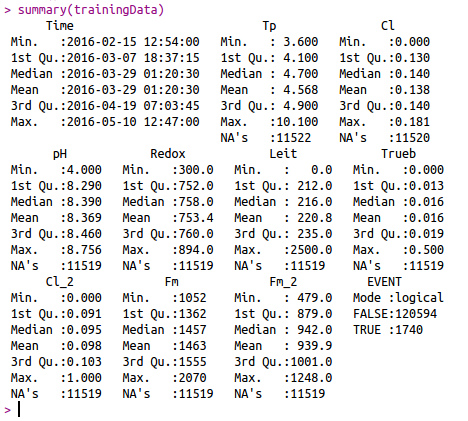
\includegraphics[width=1.2\linewidth]{trainingData.png}
\caption{Training Data Summary}
\label{fig:original}
\end{figure}

attach(trainingData)
par(mfrow=c(3,1))
trainingData$color = "black"
trainingData$color[trainingData$EVENT=="TRUE"] = "red"
plot(Cl, main="Chlorine",col=trainingData$color)
plot(Tp, main="Temperature",col=trainingData$color)
plot(pH, main="pH",col=trainingData$color)

\begin{figure}
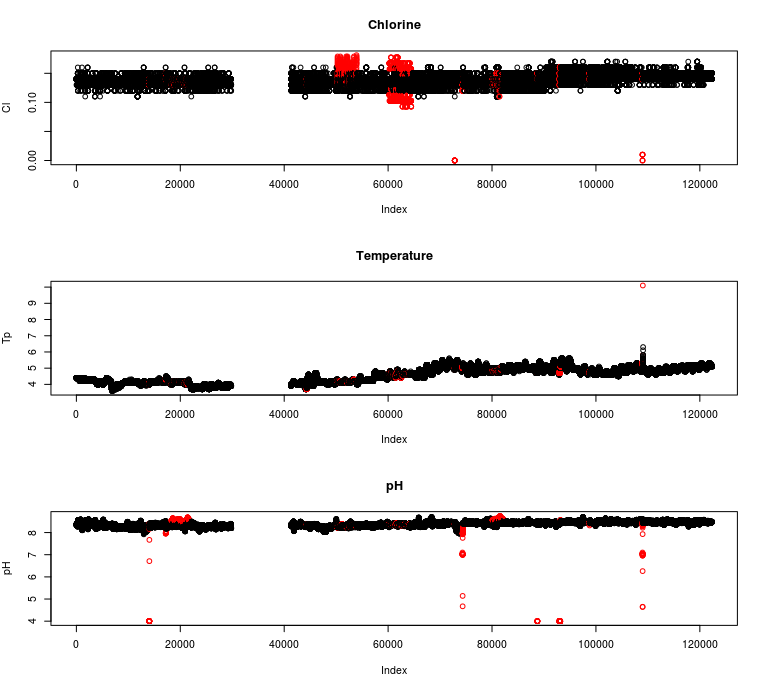
\includegraphics[width=1.2\linewidth]{Tp_Cl_pH.png}
\caption{Visualisation}
\label{fig:original1}
\end{figure}



\subsection{Definitions}
Outliers, missing values
\subsection{Implementation in R}

\section{Event Detection Algorithm}\label{sec:EDA}
\subsection{The Algorithm}

\subsection{Implementation in R}

\section{Sequential Parameter Optimization}
\subsection{Overview}
 The SPOT package can be installed from within R using the 
\begin{verbatim}
install.packages("SPOT")
\end{verbatim}
command. Alternatively, SPOT can 
downloaded from the
comprehensive R  archive network at \url{http://CRAN.R-project.org/package=SPOT}.
The latter procedure is recommended for the experienced R user only. 
SPOT is one possible implementation of the \emph{sequential parameter optimization}\/
(SPO) framework introduced in~\cite{Bart06a}.
For a detailed documentation of the functions from the SPOT package, the
reader is referred to the package help manuals.
\cite{Bart12i} introduces the SPOT and applications.
\subsection{Interfacing With Simulated Annealing}
In Figure~\ref{fig:tune2} the tuning is shown.




\section{Experiments}

\section{Results}

\section{Discussion}

\section{Summary}
Knuth says:
\cite{knuth2005art}

\bibliographystyle{splncs03}
\bibliography{ReportSample}

\end{document}